\section{Results}\label{sec:results}

% 이 절에서는 \ref{sec:methods}에서 소개한 모형들을 자료에 적용한 결과를 다룬다. 각 모형의 성능은 \citet{jeon2018additive}에서와 같이 다음과 같이 정의되는 10-fold average squared prediction error (ASPE) 값으로 비교하였다
% $$ ㅁㄹㄴㄹ $$
% . 

\subsection{Model Comparison}\label{sec:comparison}

\begin{table}
\begin{tabular}{ | p{9cm} | m{1.5cm} | } 
\hline
Method & ASPE \\
\hline
B-SBF with CBS & 5.905169 \\ 
\hline
Alpha transformation method (Tsagris(2015)) & 0.512279 \\ 
\hline
Kullback-Leibler-divergence-based regression & 0.7314985 \\
\hline
Dirichlet regression & 0.7118787 \\
\hline
Multinomial Logistic Regression & 100.0437 \\
\hline
\end{tabular}
 \caption{Comparison of ASPE}
 \label{table:1}
\end{table}

\ \quad Section \ref{sec:methods}에서 설명한 다양한 방법으로 적합하였으며, cross-validation을 통해 구한 average squared prediction error(ASPE)은 Table \ref{table:1}에 제시되어 있다. Simplex 데이터의 거리 함수... (거리함수에 대한 설명 필요) Alpha transformation method에서 alpha값은 모두 -1로 조정하였다.

ASPE를 기준으로 하였을 때, multinomial logistic을 제외한 나머지 모수적 모형들은 비교적 서로 비슷하고 준수하였다. Bochner smooth backfitting을 활용한 비모수적 모형은 이들에 비해 error가 더 크게 나타났다. Multinomial logistic의 경우 error가 지나치게 높게 계산되었는데, 이는 simplex 데이터에 극단적으로 치우친 비율이 있는 경우 수치가 조금만 차이가 나도 서로 거리가 매우 크게 계산되기 때문인 것으로 보인다.

\subsection{Visualization}\label{sec:visual}

\begin{figure}[h!]
	\centering
	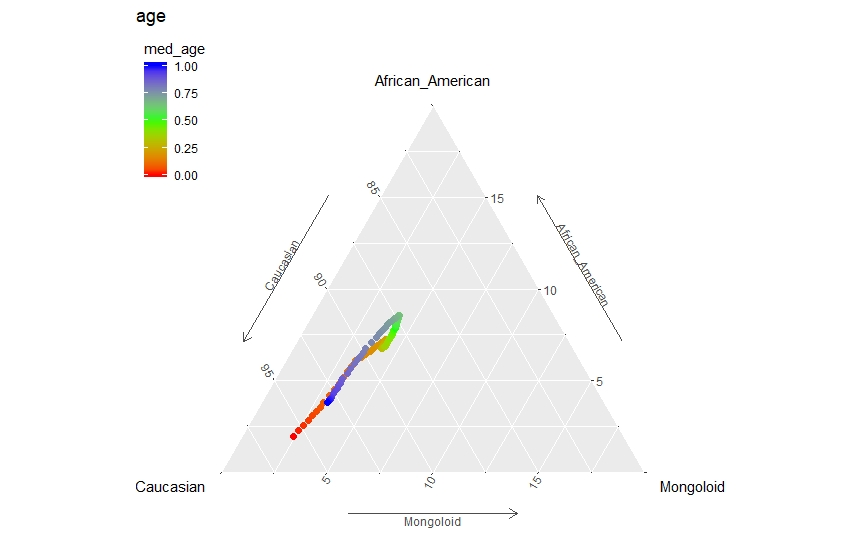
\includegraphics[width=0.48\linewidth]{figs/p_age.jpeg}
	\hspace{.005\linewidth} 
	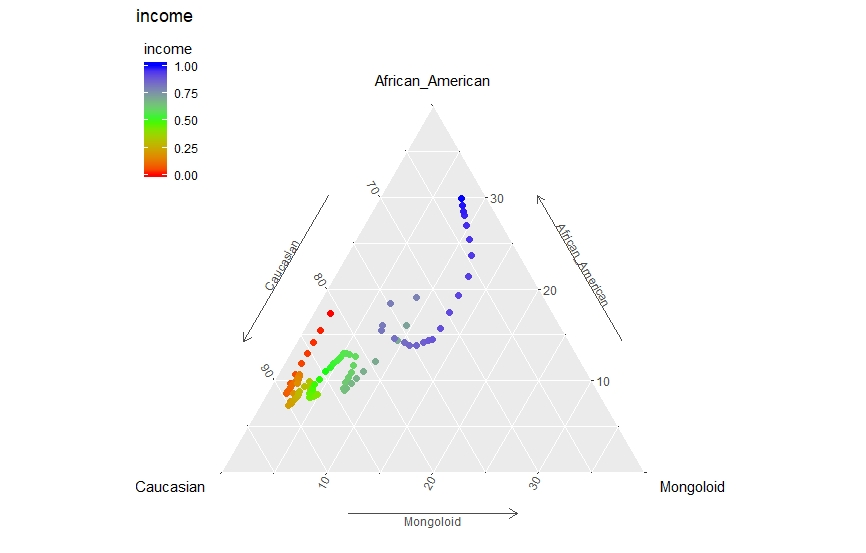
\includegraphics[width=0.48\linewidth]{figs/p_income.jpeg}
	\\[.5\baselineskip]
	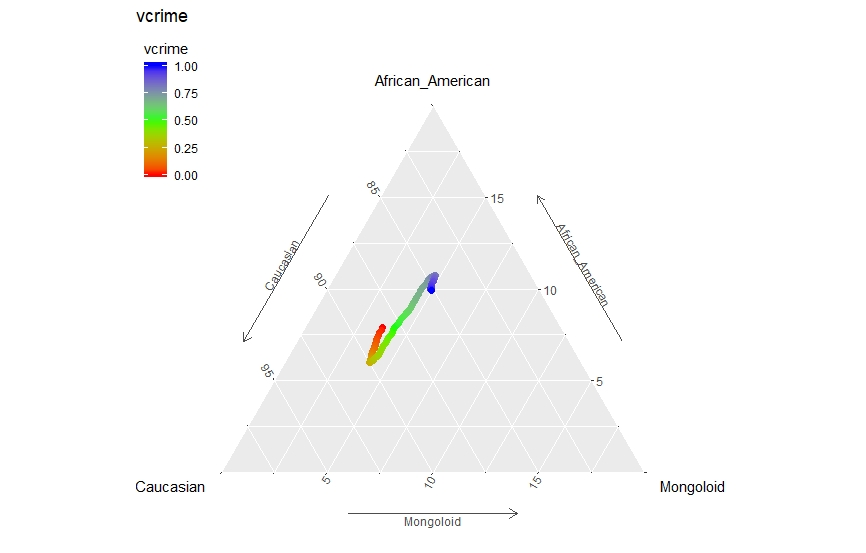
\includegraphics[width=0.48\linewidth]{figs/p_vcrime.jpeg}
	\hspace{.005\linewidth} 
	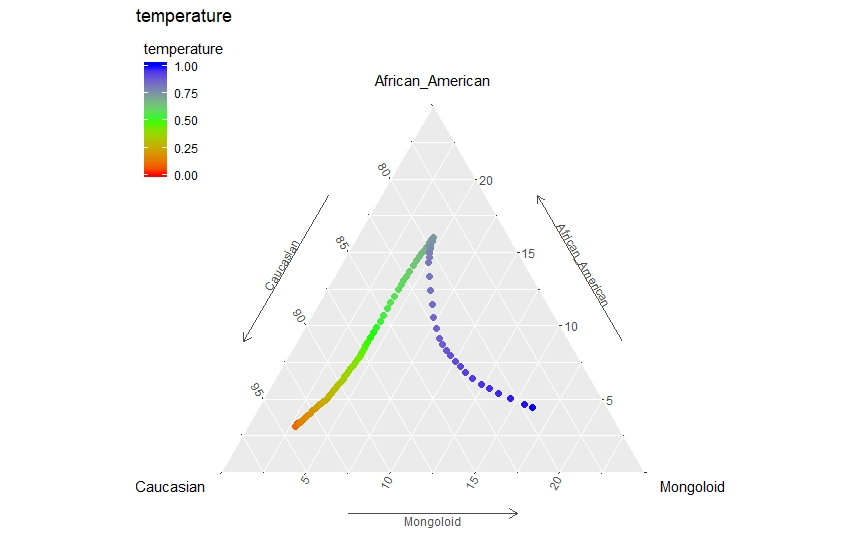
\includegraphics[width=0.48\linewidth]{figs/p_temperature.jpeg}
	\\[.5\baselineskip]
	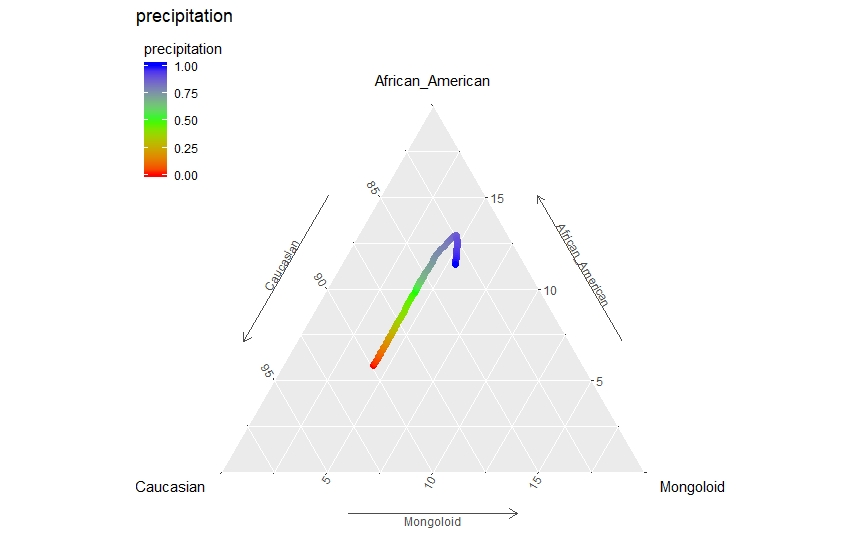
\includegraphics[width=0.48\linewidth]{figs/p_precipitation.jpeg}
	\caption{\citet{jeon2018additive}의 방법을 이용하여 적합한 인구 구성비 결과를 나타낸 2-simplex (ternary diagram) visualization.}
\end{figure}

\ \quad Figure 1은  \citet{jeon2018additive}에서 제시된 방법을 이용해서 적합한 성분비의 추정 값들이 각 요인들의 움직임에 따라 어떻게 움직이는 지를 시각화한 것이다. 각각의 요인들의 영향력을 알아보기 위해서 우리는 성분비의 추정 값을 계산할 때 정해진 한 변수를 제외하고 다른 변수들은 모두 평균값으로 세팅하였고, 한 변수 값의 움직임에 따라 어떻게 성분비의 추정 값이 변화하는 지를 분석해 보았다. 

첫 번째 그림에서는 연령대가 변화함에 따라서 인구 구성비 중에서 흑인과 백인의 비율이 두드러지게 변화한다는 것을 알 수 있다. 연령대가 높아짐에 따라서 처음에는 백인의 비율이 감소하고 흑인의 비율은 증가하다가 일정 나이대를 지나면 다시 백인의 비율이 증가하고 흑인의 비율은 증가하는 경향을 보이고 있다. 여기서 동양인의 비율은 평균 연령대가 변화해도 크게 변동하지 않는다는 흥미로운 사실을 발견하였다. 

두 번째 그림은 수입이 변화함에 따라서 인구 구성비가 어떻게 변화하는지를 보여주고 있다. 다른 4개의 요인에 비해 불규칙한 경향성을 보이고 있다. 다만 전반적으로 평균 수입이 늘어남에 따라서 동양인의 비율이 늘어나고 흑인의 비율은 줄어드는 경향을 보이고 있다. 또한, 일정 수준 이상부터는 수입이 늘어남에 따라 백인의 비율이 줄어드는 경향성을 보인다. 수입 최상위층 구간에서 흑인의 비율이 조금 늘어나고 동양인의 비율은 오히려 줄어드는 경향을 보이는 것이 또 하나의 흥미로운 사실이었다.

세 번째 그림에서는 범죄율이 변함에 따라서 흑인과 백인의 비율이 두드러지게 변화하는 것을 알 수 있다. 양 극단을 제외하고는 범죄율이 높을수록 흑인의 비율이 늘어나고 백인의 비율은 줄어들지만, 극단에서는 이 관계가 역전이 되고 있다. 한편 동양인의 비율은 범죄율에 거의 영향이 없는 것으로 보였다. 

네 번째 그림, 다섯 번째 그림은 각각 온도, 강수량의 변화에 따른 인구 구성비의 변화를 나타낸다. 일정 온도 이하까지는 온도가 높아질수록 흑인의 비율은 늘어나고 백인의 비율은 줄어들다가, 일정 온도 이상이 되면 흑인의 비율은 줄어들고 동양인의 비율은 두드러지게 늘어남을 알 수 있다. 이는 알래스카와 같은 척박한 곳에는 백인의 비율이 높지만 일정 온도 이상이 되면 온도가 오를 수록, 즉 살기에 더 쾌적할수록 동양인의 비율이 늘어나고 있음을 보여주고 있다. 강수량에 따른 변화 역시 비슷한 경향을 보인다. 즉, 강수량이 낮은 구간에서는 백인의 비율이 높지만 일정 강수량 이상이 되는 지점부터는 강수량이 늘어날수록 동양인의 비율이 높아지고 있다.

% 실험과 관련된 코드는 github repository \url{https://github.com/kw-lee/ARHR_USA}에 제공되어 있다.
